%%%%%%%%%%%%%%%%%%%%%%%%%%%%%%%%%%%%%%%%%
% University/School Laboratory Report
% LaTeX Template
% Version 3.1 (25/3/14)
%
% This template has been downloaded from:
% http://www.LaTeXTemplates.com
%
% Original author:
% Linux and Unix Users Group at Virginia Tech Wiki 
% (https://vtluug.org/wiki/Example_LaTeX_chem_lab_report)
%
% License:
% CC BY-NC-SA 3.0 (http://creativecommons.org/licenses/by-nc-sa/3.0/)
%
%%%%%%%%%%%%%%%%%%%%%%%%%%%%%%%%%%%%%%%%%

%----------------------------------------------------------------------------------------
%	PACKAGES AND DOCUMENT CONFIGURATIONS
%----------------------------------------------------------------------------------------

\documentclass{article}

\usepackage[version=3]{mhchem} % Package for chemical equation typesetting
\usepackage{siunitx} % Provides the \SI{}{} and \si{} command for typesetting SI units
\usepackage{graphicx} % Required for the inclusion of images
\usepackage{natbib} % Required to change bibliography style to APA
\usepackage{amsmath} % Required for some math elements 
%\usepackage{url}
\usepackage{hyperref}
\usepackage{subcaption}
\usepackage{float}
\usepackage{array}



\setlength\parindent{0pt} % Removes all indentation from paragraphs

%\renewcommand{\labelenumi}{\alph{enumi}.} % Make numbering in the enumerate environment by letter rather than number (e.g. section 6)

%\usepackage{times} % Uncomment to use the Times New Roman font

%----------------------------------------------------------------------------------------
%	DOCUMENT INFORMATION
%----------------------------------------------------------------------------------------

\title{Homework \#4 \\Elliptic Curves \\[0.2em]\small{}CNS Course Sapienza} % Title and subtitle

\author{Riccardo \textsc{Prinzivalle}, 1904064} % Author name

\date{November 20, 2020} % Date for the report

\begin{document}

\maketitle % Insert the title, author and date

%----------------------------------------------------------------------------------------
%	SECTION 0
%----------------------------------------------------------------------------------------

\section{Homework Goal}

This homework contains a basic python implementation of AES algorithm. Throughout the work, it has been chosen to make a compromise: the implementation is in midpoint between complete Galois Field and precomputed look-up tables for every step. Both encryption and decryption are studied and implemented, then the operation modes are implemented and finally it will illustrate a comparison with world known AES implementation.

\begin{table}[H]
\begin{center}
\begin{tabular}{ll}
Input text &  6bc1bee22e409f96e93d7e117393172a\\
	      &   ae2d8a571e03ac9c9eb76fac45af8e51\\
	      &   30c81c46a35ce411e5fbc1191a0a52ef\\
	      &   f69f2445df4f9b17ad2b417be66c37 \\
\\
Key & 2b7e151628aed2a6abf7158809cf4f3c\\
\\
IV (where needed) & 5468617473206D79204B756E67204675
\end{tabular}
\caption{Parameter used in testing of AES operation modes}
\label{tab:AESparameter}
\end{center}
\end{table}

%----------------------------------------------------------------------------------------
%	SECTION 1
%----------------------------------------------------------------------------------------

\section{Mathematical background}
 

%----------------------------------------------------------------------------------------
%	SECTION 2
%----------------------------------------------------------------------------------------

\section{Discrete Logarithm Problem with Elliptic Curves}


\begin{figure}[H]
\centering
\begin{subfigure}{.54\textwidth}
  \centering
  %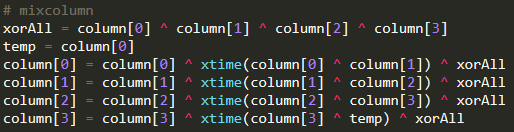
\includegraphics[width=1\linewidth]{images/mixcolumn.png}
  \caption{Core}
  \label{fig:core}
\end{subfigure}
\begin{subfigure}{.35\textwidth}
  \centering
  %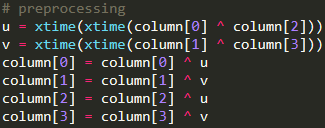
\includegraphics[width=1\linewidth]{images/preprocessing.png}
  \caption{Preprocessing}
  \label{fig:preprocessing}
\end{subfigure}
\caption{Mix columns base functions}
\label{fig:MixColumns}
\end{figure}
 
%----------------------------------------------------------------------------------------
%	SECTION 3
%----------------------------------------------------------------------------------------

\section{Use of Elliptic Curves in Cryptography}


%----------------------------------------------------------------------------------------
%	SECTION 4
%----------------------------------------------------------------------------------------

\section{Conclusion}

Even if the implementation proposed is much slower than the standard library chosen as comparison, it works well and it does its dirty job. The code may not be much optimized or it can have been written in a better way but my knowledge in python is not so huge, but this was an opportunity to dust and improve my experience.


%----------------------------------------------------------------------------------------
%	BIBLIOGRAPHY
%----------------------------------------------------------------------------------------

\bibliographystyle{abbrv}

%\bibliography{sample}

%----------------------------------------------------------------------------------------


\end{document}